\documentclass{article}

\usepackage{amsmath}
\usepackage{amsthm}
\usepackage{amssymb}
\usepackage{color}
\usepackage{tikz}
\usetikzlibrary{shapes,arrows}
\usepackage{etoolbox}
\usepackage{url} % for urls in bibliography
\usepackage[parfill]{parskip} % no paragraph indents, leave blank line
\usepackage{graphicx}
\usepackage{subcaption}
\usepackage{listings}


\graphicspath{ {./drawio/} }

% Need this to keep the space before theorems when using parfill parskip
% https://tex.stackexchange.com/questions/25346/wrong-spacing-before-theorem-environment-amsthm
\begingroup
    \makeatletter
    \@for\theoremstyle:=definition,remark,plain\do{%
        \expandafter\g@addto@macro\csname th@\theoremstyle\endcsname{%
            \addtolength\thm@preskip\parskip
            }%
        }
\endgroup

\DeclareRobustCommand{\rchi}{{\mathpalette\irchi\relax}}
\newcommand{\irchi}[2]{\raisebox{\depth}{$#1\chi$}} % inner command, used by \rchi

\title{Nitro Protocol}
\author{Tom Close}

\usepackage{mathtools}
\usepackage{bm}
\usepackage{stmaryrd} % for llbracket and rrbracket

\theoremstyle{definition}
\newtheorem{example}{Example}[section]
\newtheorem{defn}{Definition}[section]

\newcommand{\adj}[1]{\llbracket #1 \rrbracket} 
\newcommand{\enf}[1]{[#1]} 

\begin{document}

\maketitle

\section{Introduction}

A blockchain is a device that enables a group of adversarial parties to come to consensus over the contents of a shared ledger, without appealing to a trusted central authority. 
Whether using a proof-of-work or a proof-of-stake algorithm, this process has a cost both in terms of time and in terms of money.
For the Ethereum blockchain, this cost results in an effective limit of around 15 transactions per second being processed on the network.
When compared with the visa network, which can process on the order of 50,000 transactions per second, this limit supports the view that blockchains, in their current form, do not scale.

State channels offer a solution to the blockchain scaling problem.
A state channel can be thought of as a set of updatable agreements between a fixed set of participants determining how a given set of assets should be split between them.
The agreements are updated off-chain through the exchange of cryptographically signed messages between the participants according to some set of previously-agreed update rules. 
The assets in question are held in escrow on the blockchain, in such a way
that they can only be released according to the latest agreement from the state channel.
If the off-chain cooperative behaviour breaks down, for example if one party refuses to sign updates either by choice or due to unavailability, any of the parties can reclaim their share of the assets by presenting the latest agreement to the chain.
An exit game is required to give other parties the opportunity to present a later state, but all parties have the guarantee that they can reclaim their share of the funds within some finite time.

In addition to the increased throughput, state channels bring instant finality to transactions: the moment a channel update is received the participant knows that the assets transferred are now assigned to them.
They cannot access the assets immediately but they have the power to prevent any other party claiming those assets in the future.
The only requirement is that participants need to be live enough to engage in the exit game if an opponent attempts to exit an earlier state.
In practice, the requirement here is to check the chain periodically - at time intervals that are less than, but on the same order of magnitude as, the challenge duration in the exit game.

As the channel updates are created and exchanged off-chain, the channel-update throughput is limited only by the speed of constructing, signing and broadcasting the update.
Given that channel updates only needed to be communicated between participants and the system is therefore highly parallelizable, it is difficult to put a bound on the total transaction throughput of a system of state channels.
In practice the system is only limited by the on-chain operations required to move assets when opening and closing channels.

In this paper, we allow channels to be opened and closed off-chain. We enable the construction of efficient state channel networks.[TODO]

\section{Existing work}

Lightning and raiden
- payment channel networks
- directional

Celer
- directional but with multiple paths
- general conditions

Perun
- virtual payment channels (different from HTLCs)
- but using a validity time
- and then state channel networks
[Connext - have removed the time limit with a trade-off of trusting the hub - TODO: check this]

Counterfactual
- thinks about counterfactual instantiation
- also app instance on top, which we collaborated on
- possible to do meta-channels, but the details are not given in the paper and are still being finalized

Our contribution:
- like perun without the time limit
Unconstrained subchannels

\section{State Channel Concepts}



- abstract away a lot of the details
- one type of coin
- ForceMove centric but believe that the ideas presented here, in some form, are present in most frameworks
- draw examples from ForceMove: turn based, programmable by specifying libraries

- signature scheme
- hash

\subsection{Participants and Addresses}

- in this paper we will deal with systems of interacting state channels
- it will be useful to start by looking at some of the parameters that give these
   systems their characteristics
- in particular we will look at three important parameters: the space of participants,
  the space of assets and the application rules

- consider a state channel system (Participants, Assets, ApplicationRules)

- space of participant addresses
- all addresses generated from the signature scheme
- someone somewhere should know the private key corresponding to a participant address
- they are the owner of that address
- a participants can own multiple addresses
- the key is used to sign updates
- addresses don't have to have any funds allocated on-chain - they can be ephemeral

- space of channels
- ordered subset of participants
- a nonce
- channel address
- 

- space of assets
- allowed values these can take
- in this paper we deal with a single asset which we will refer to as coins
- the assets allocated can be summarised with a single integer
- in this paper we allow the coin value to take any value in $\mathbb{Z}$
- this is not realistic for the blockchain context, where there is typically a maximum
  value, \texttt{MAX}, after which totals overflow
- meaning that we should really consider coins in the space $\mathbb{Z}_{\texttt{MAX}}$
- in ethereum $\texttt{MAX} = 2^{256} - 1$
- we can also consider state channels that operate on multiple assets: $\mathbb{Z}_{\texttt{MAX}} \times \mathbb{Z}_{\texttt{MAX}}$

- space of application rules. Consider these to also define the states
- state transitions
- payment channel can be thought of in terms of a state channel system with a single application
- is it possible to add to the space of application rules
- what sort of rules does it support? transition rules depend on time or the general state of the chain
- we assume here that they don't
- possible to remove these restrictions



- space of channel addresses
- participant addresses
- channels = set of participants + nonce
- channel addresses

\subsection{Funding and Channel Outcomes}

- adjudicator: two important collections - funds held and outcomes
- holding funds + notation
- holding outcomes

- outcomes of a channel
- outcome: how funds should be distributed
- notation
- make this precise later


- ways of registering outcomes in force move
- only one outcome on-chain for each channel. Once one outcome has been registered no other one can be
- abstract a channel to be something that can reach an outcome

- first part of this is what outcomes you can register on-chain

\subsection{Finalizable and Enabled Outcomes}

- state of a channel
- outcome is finalizable if you can register it on-chain and no-one can stop you.
- an unbeatable strategy for getting it on-chain
- series of actions

\begin{example}{The next mover in ForceMove.}
  In a ForceMove state channel with $n$ participants, if participant $p$ has just received state $\sigma_m$ with $m > n$ and it is their turn to sign state $m+1$, then we have $\enf{\sigma_m.\beta}_p$ - the state's balances $\sigma_m.\beta$ is a finalizable outcome for $p$.
  Why? To finalize this outcome $p$ can call a force-move on $\sigma_m$ and then fail to respond within
  the timeout. [The reason why ForceMove always allows a transition to a conclude state is to
  give $p$ a way of accomplishing the same outcome off-chain.]
\end{example}

\begin{example}{Two conclusion proofs.}
  In a ForceMove state channel, if two different conclusion proofs with different outcomes,
  $\beta_1 \neq \beta_2$, are both held by participants $p_1$ and $p_2$, then no outcome is finalizable by any participant.
  Why? No finalizable outcome other than $\beta_1$ is possible any party $p$, as it is always
  possible for either $p_1$ or $p_2$ to register the conclusion proof resulting $\beta_1$ immediately.
  But the same is also true for $\beta_2$. Therefore no finalizable outcome exists.
  [For this reason, participants should never sign more than one conclusion state.]
\end{example}

- enabled outcomes

\begin{example}{Pre-fund setup in ForceMove.}
  In a ForceMove state channel with $n$ participants $P$, at end of the pre-fund setup i.e.
  when the last state to be broadcast was $\sigma_n$, then we have $\enf{\sigma_n.\beta}_P$ -
  the state's balances $\sigma_n.\beta$ is finalizable for all participants of the channel.
  Why? According to the ForceMove transition rules, the outcome must remain unchanged for the
  first $2n$ states. That means that every participant must contribute another signature before
  the outcome of the state can change. By with-holding this signature and forcing the channel to
  conclusion through a series of force-moves, any participant can ensure that the current
  outcome is registered on-chain.
\end{example}

\subsection{Systems of Channels}

- system: related channels + adjudicator
- value (unbeatable strategy for extracting at least a given total, without assuming we add funds)
- value equivalent (if two system states have the same value)
- value preserving transition
- transitioning between outcomes
- rewrite rules
- channels update independently

- possible to transition between finalizable states

\section{Turbo Protocol}

Turbo protocol allows a set of participants who already have a funded channel to open and
close sub-channels without any on-chain transactions. 

As an example, suppose Alice and Bob want to play a game of chess and that
they already have an existing state channel, $\rchi_L$, which holds
5 of Alice's coins and 5 of Bob's.
2 coins from the loser.

\begin{center}
  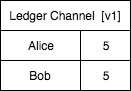
\includegraphics[scale=0.5]{turbo_start} % TODO: tikz
\end{center}

They decide that winner of the chess game should win 2 coins from the loser and proceed
by creating a new channel $\rchi_C$ for the chess game with the appropriate starting state.
They then update $\rchi_L$ to allocate funds to these games.

\begin{center}
  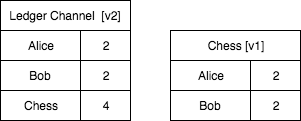
\includegraphics[scale=0.5]{turbo_open} %TODO: tikz
\end{center}

Once the funds are allocated, they are free to play the game of chess.
Updates to the chess channel are independent from updates to $\rchi_L$ and to
any other sub-channels that are potentially funded by it. 
Alice wins the chess game, so the final state in the chess channel allocates all the
funds to her.

\begin{center}
  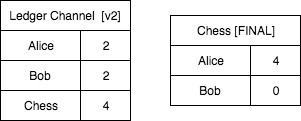
\includegraphics[scale=0.5]{turbo_close} %TODO: tikz
\end{center}

To close the chess channel off-chain, Alice and Bob update the state of the ledger channel to absorb the outcome of the game.

\begin{center}
  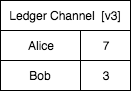
\includegraphics[scale=0.5]{turbo_finish} %TODO: tikz
\end{center}

In the rest of this section we will present the protocol that makes the above interaction
possible.

\subsection{Constructing Turbo}

The key difference between Turbo and ForceMove is that Turbo allows the outcome of a channel to allocate funds to other \textit{channels}, as well as to the participants.

While this generalization allows for a variety of relationships between different channels,
we will focus here on a setup where a single parent channel funds one or more sub-channels
\footnote{Note that we allow the case where the sub-channels are themselves ledger channels.}.
Following the Perun paper, we will refer to this parent channel as a \textbf{ledger channel}.

Interpretation and manipulation of the outcomes when they exist on-chain. Registering those
outcomes is done by ForceMove.

\begin{center}
  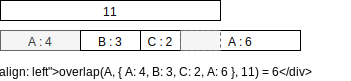
\includegraphics[scale=0.7]{overlap} % TODO: tikz
\end{center}
\lstinputlisting[language=Python]{code/overlap.py}

\begin{center}
  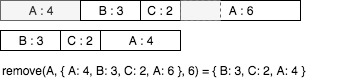
\includegraphics[scale=0.7]{remove} % TODO: tikz
\end{center}
\lstinputlisting[language=Python]{code/remove.py}

We will now introduce the three on-chain operations that drive Turbo: deposit, withdrawal,
and transfer.


The \textbf{deposit} operation is used to increase the funds held for a given channel.
In order for the operation to be valid it must be accompanied by a transfer of funds equal 
to the increase.
\begin{align*}
D_\rchi(x) \adj{\alpha_\rchi(y)} = \adj{\alpha_\rchi(x + y)}
\end{align*}
The deposit can be called by anyone but a rational participant, $p$, should only make a
deposit of size $x$ if it causes the value of the system state for $p$ to increase by $x$.

The \textbf{withdrawal} operation is used to withdraw funds held at a given 
address, $A$, by a party with a knowledge of the corresponding private key. If $x \leq x'$ then
\begin{align*}
W_A(x) \adj{\alpha_A(x')} = \adj{\alpha_A(x'-x)}
\end{align*}
In the above equation, we focus only on the affect of the withdrawal operation on the system state.
In practice the withdrawal should also specify the external address that the funds should be sent to
along with the signature.
A potential method signature is \texttt{withdraw(fromAddr, toAddr, amount, signature)}, 
where \texttt{signature} is $A$'s signature of the other parameters
\footnote{In practice, we can add the \texttt{senderAddress} to the parameters to sign,
in order to prevent replay attacks.}.
Note that the signature requirement coupled with the no-collision assumption means
it is not possible to withdraw from the funds held for a channel.

The \textbf{transfer} operation, $T_{A,B}(x)$, is an instruction to transfer funds currently allocated
to address $A$ to address $B$, according to the outcome of channel $A$.

\lstinputlisting[language=Python]{code/transfer.py}

If channel $X$ holds x and the outcome of $X$ allocates $y$ to $Y$ within $x$.
- then update channel X to hold x, channel Y to hold y, and decrease the amount X allocates to Y by y

For example, 
\begin{align*}
T_{A,B}(3) \adj{\alpha_A(10)\beta_A(B: 3, C: 7)} = \adj{\alpha_A(7)\alpha_B(3)\beta_A(C: 7)}
\end{align*}

\subsection{Value Equivalence in Turbo}

- transfer operations commute
- value equivalent in terms of $\alpha_A$
- if I can find one set of transfer operations they're equivalent

- 

- funding a ledger channel - only deposit if it increases your value by the deposit amount
- opening a subchannel

\subsection{Examples}


\subsubsection{Opening a sub-channel}

\begin{align*}
  S_1 &= \adj{\alpha_L(a+b)} &&\enf{\beta_L(A: a, B: b)}_{A, B} & \\
  S_2 &= \adj{\alpha_L(a+b)} &&\enf{\beta_L(A: a, B: b)}_{A, B}&\enf{\beta_\rchi(A: a', B: b')}_{A, B} \\
  S_3 &= \adj{\alpha_L(a+b)} &&\enf{\beta_L(A: a-a', B: b-b', \rchi: a' + b')}_{A, B}&\enf{\beta_\rchi(A: a', B: b')}_{A, B}
\end{align*}

\subsubsection{Closing a sub-channel}

\begin{align*}
S_1 &= \adj{\alpha_L(x)} &&\enf{\beta_L(A: a, B: b, \rchi: a' + b')}_{A, B}&\enf{\beta_\rchi(A: a', B: b')}_{A, B}\\
S_2 &= \adj{\alpha_L(x)} &&\enf{\beta_L(A: a + a', B: b + b')}_{A, B}&\enf{\beta_\rchi(A: a', B: b')}_{A, B} \\
S_3 &= \adj{\alpha_L(x)} &&\enf{\beta_L(A: a + a', B: b + b')}_{A, B} & 
\end{align*}
where $x = a + a' + b + b'$.

\subsubsection{Topping up a ledger channel}

\begin{align*}
S_1 &= \adj{\alpha_L(a + b)} &&\enf{\beta(A: a, B: b)}_{A, B} \\
S_2 &= \adj{\alpha_L(a + b)} &&\enf{\beta(B: b, A: a + a')}_{A, B} \\
S_3 &= D_L(a')\adj{\alpha_L(a + b)} &&\enf{\beta(B: b, A: a + a')}_{A, B} \\
S_4 &= \adj{\alpha_L(a + b + a')} &&\enf{\beta(B: b, A: a + a')}_{A, B}
\end{align*}

\subsubsection{Partial checkout from a ledger channel}

\begin{align*}
S_1 &= \adj{\alpha_L(x)} &&\enf{\beta_L(B: b, A: a, \rchi: c)}_{A, B} & \\
S_2 &= \adj{\alpha_L(x)} &&\enf{\beta_L(B: b, A: a, \rchi: c)}_{A, B} & \enf{\beta_{L'}(B: b, A: a - a', \rchi: c)}_{A, B}\\
S_3 &= \adj{\alpha_L(x)} &&\enf{\beta_L(L': x-a', A: a)}_{A, B} & \enf{\beta_{L'}(B: b, A: a - a', \rchi: c)}_{A, B}\\
S_4 &= \adj{\alpha_L(x)\beta_L(L': x-a, A: a)} && & \enf{\beta_{L'}(B: b, A: a - a', \rchi: c)}_{A, B}\\
S_5 &= \adj{\alpha_L'(x-a)\alpha_A(a)} && & \enf{\beta_{L'}(B: b, A: a - a', \rchi: c)}_{A, B}\\
\end{align*}

\section{Nitro Protocol}

- virtual channels
- quick sketch

- guarantee outcomes + on-chain operation

- construction

- opening + closing


\section{Acknowledgements}

- Andrew Stewart
- James Prestwich
- Chris Buckland
- Magmo team


\section{Appendix}

\subsection{Overview of ForceMove}
\subsection{The Consensus Game}
\subsection{Virtual Channels on Turbo}
\subsection{Payouts to Non-Participants}
\subsection{Possible Extensions}


\end{document}
